\chapter{Modelling Limit Order Books Using Hawkes Processes}

In the previous chapters, we have seen LOB models dominated by Poisson processes, which assume that order arrivals are completely independent of one another. However, this assumption contradicts the reality of financial markets. Standard Poisson models fail to replicate critical microstructural phenomena, such as \textbf{volatility clustering} and \textbf{correlated order flow}.

\begin{itemize}
    \item\textbf{Volatility clustering} in a limit order book refers to the tendency of large price changes to occur in bursts, followed by periods of relative calm. This arises because liquidity in the book is not constant. When the available depth at the best bid and ask is low, incoming orders have a larger price impact. During periods of heavy trading or uncertainty, limit orders are often cancelled and spreads widen, making the book thinner. As a result, successive trades move prices more, leading to sustained periods of high volatility.
    \begin{figure}[h]
        \centering
        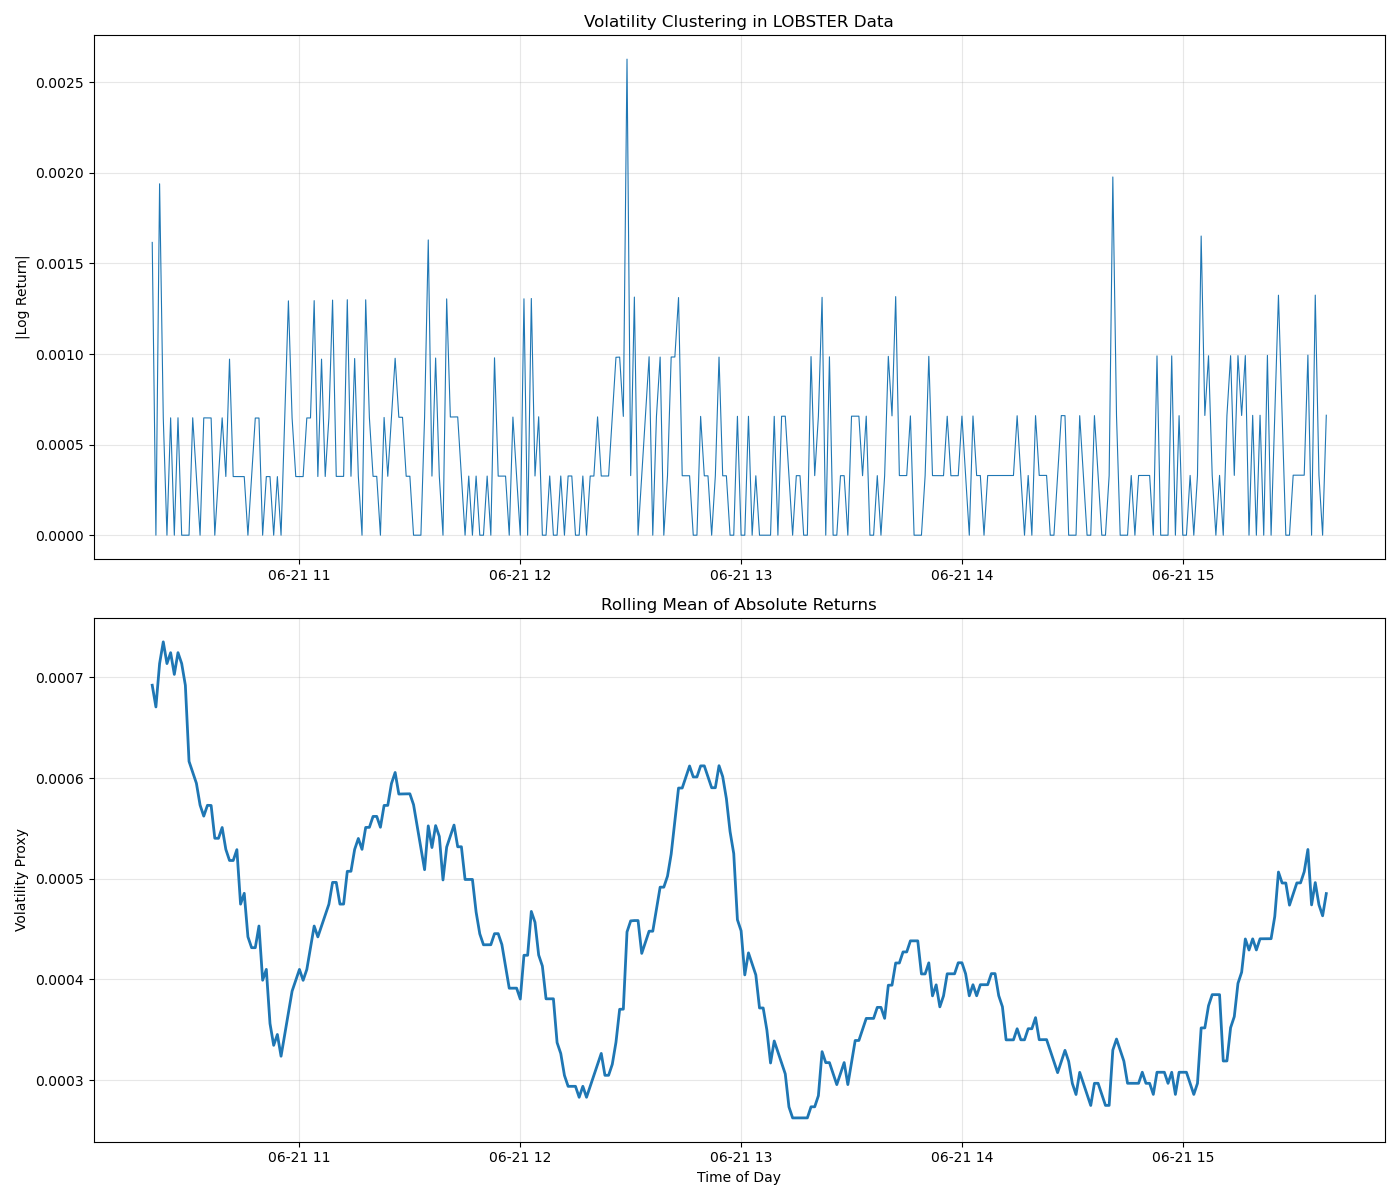
\includegraphics[width=0.82\linewidth]{Volatility Clustering.png}
        \caption{\textit{Volatility Clustering shown by MSFT Stock on 21st Jun. 2012.} Figure depicts clear periods of high volatility followed by periods of low volatility}
        \label{fig:volclustering}
    \end{figure}
    
    \item \textbf{Correlated order flow} refers to the persistence in the direction of trades, where buy orders are likely to be followed by more buy orders, and similarly for sell orders. This occurs due to order splitting by large traders, algorithmic execution strategies, and common reactions to information. In a limit order book, such persistent order flow repeatedly consumes liquidity on one side, causing prices to move in that direction. 
    \begin{figure}[h]
        \centering
        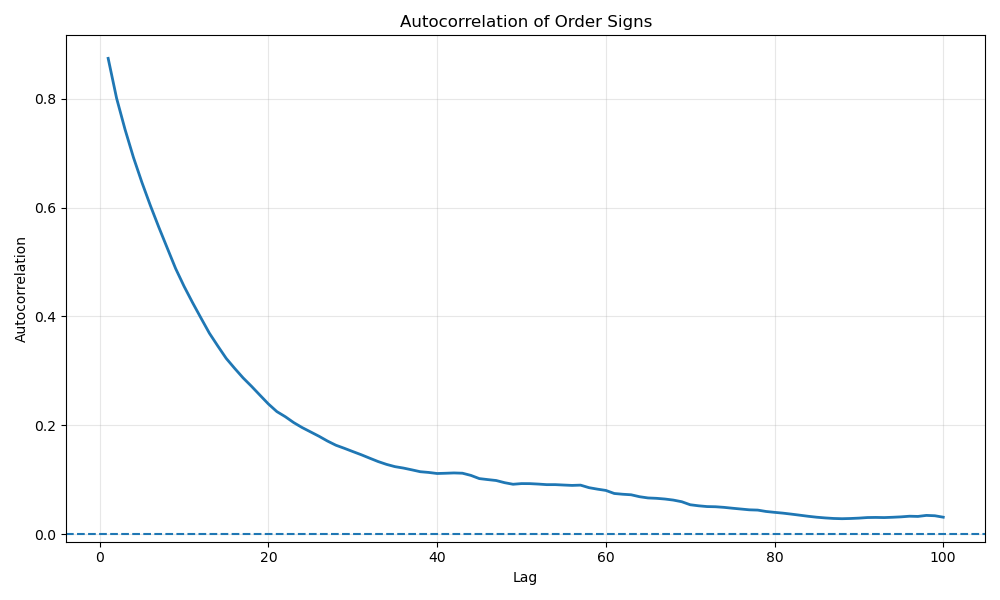
\includegraphics[width=0.82\linewidth]{Autocorrelation.png}
        \caption{\textit{Correlation between orders shown by MSFT Stock on 21st Jun. 2012}. For short lags, a high correlation is seen between orders}
        \label{fig:autocorrelation}
    \end{figure}
\end{itemize}

Here, the Hawkes process presents a compelling mathematical alternative. By dropping the strict requirement for independent increments, it treats order flow as an endogenously excited process, meaning that past events can trigger future ones. This subtle shift allows the model to replicate both volatility clustering and correlated order flows. Hawkes processes also possess the advantage of being mathematically descriptive, as opposed to the 'black boxes' of deep learning models. They offer complete transparency, allowing researchers to see and explain the mechanics driving the simulation.

However, applying standard Hawkes models directly to LOB dynamics has its challenges. 
\begin{itemize}
    \item \textbf{Constant Order Sizes:} Standard Hawkes models focus primarily on capturing inter-event times, assuming order sizes remain constant. In reality, empirical distributions show significant spikes at round numbers (e.g., 100, 500), reflecting traders' preferences.
    \item \textbf{Negative Spreads:} The bid-ask spread in an exchange can never be mathematically less than one tick, a mechanical constraint that standard point processes may violate.
    \item \textbf{Inhibitory Excitations:} Cross-excitations between certain events (like limit orders inside the spread and cancellations) can be inhibitory, potentially introducing mathematically invalid negative intensities into the point process.
    \item \textbf{Intraday Seasonality:} Order intensities exhibit a stationary ``U''-shape throughout the trading day (high activity near open and close), which must be accounted for.
\end{itemize}
\begin{figure}[h]
    \centering
    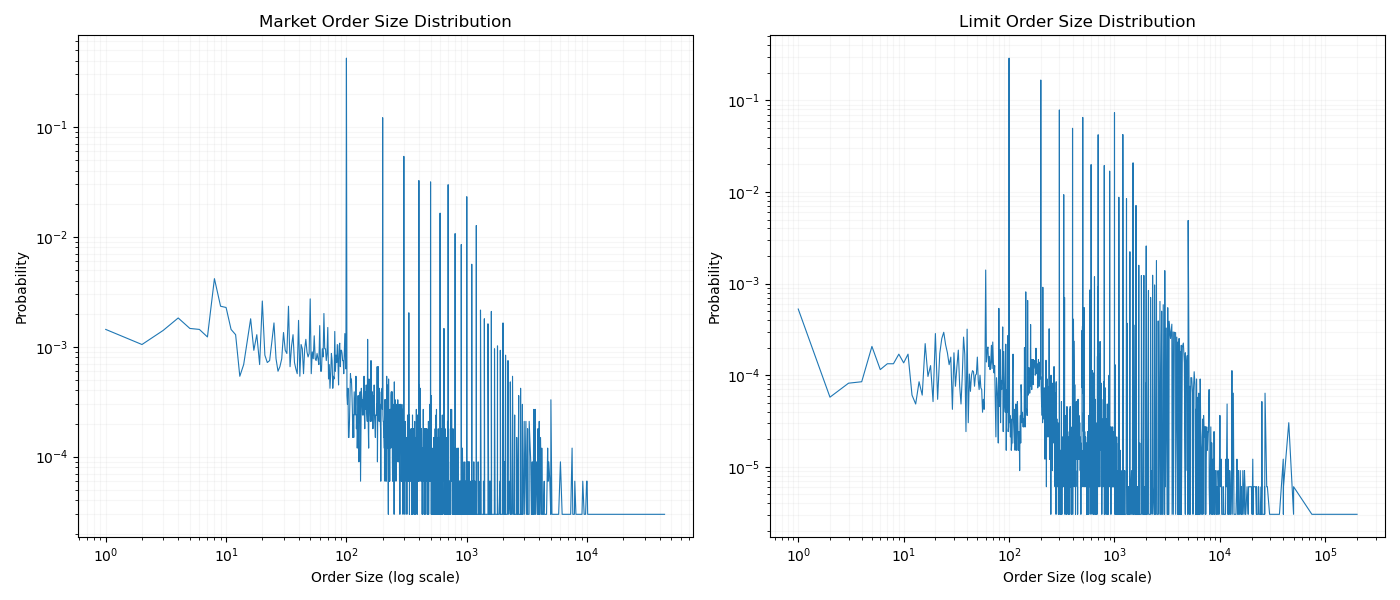
\includegraphics[width=0.82\linewidth]{Size Distribution.png}
    \caption{\textit{(log-log) Empirical Distribution of Order Sizes of 
    MSFT Stock on 21st Jun. 2012}. A high spike is seen on order sizes of round numbers such as 100/500/1000}
    \label{fig:ordersizesmsft}
\end{figure}
% \begin{figure}[h]
%     \centering
%     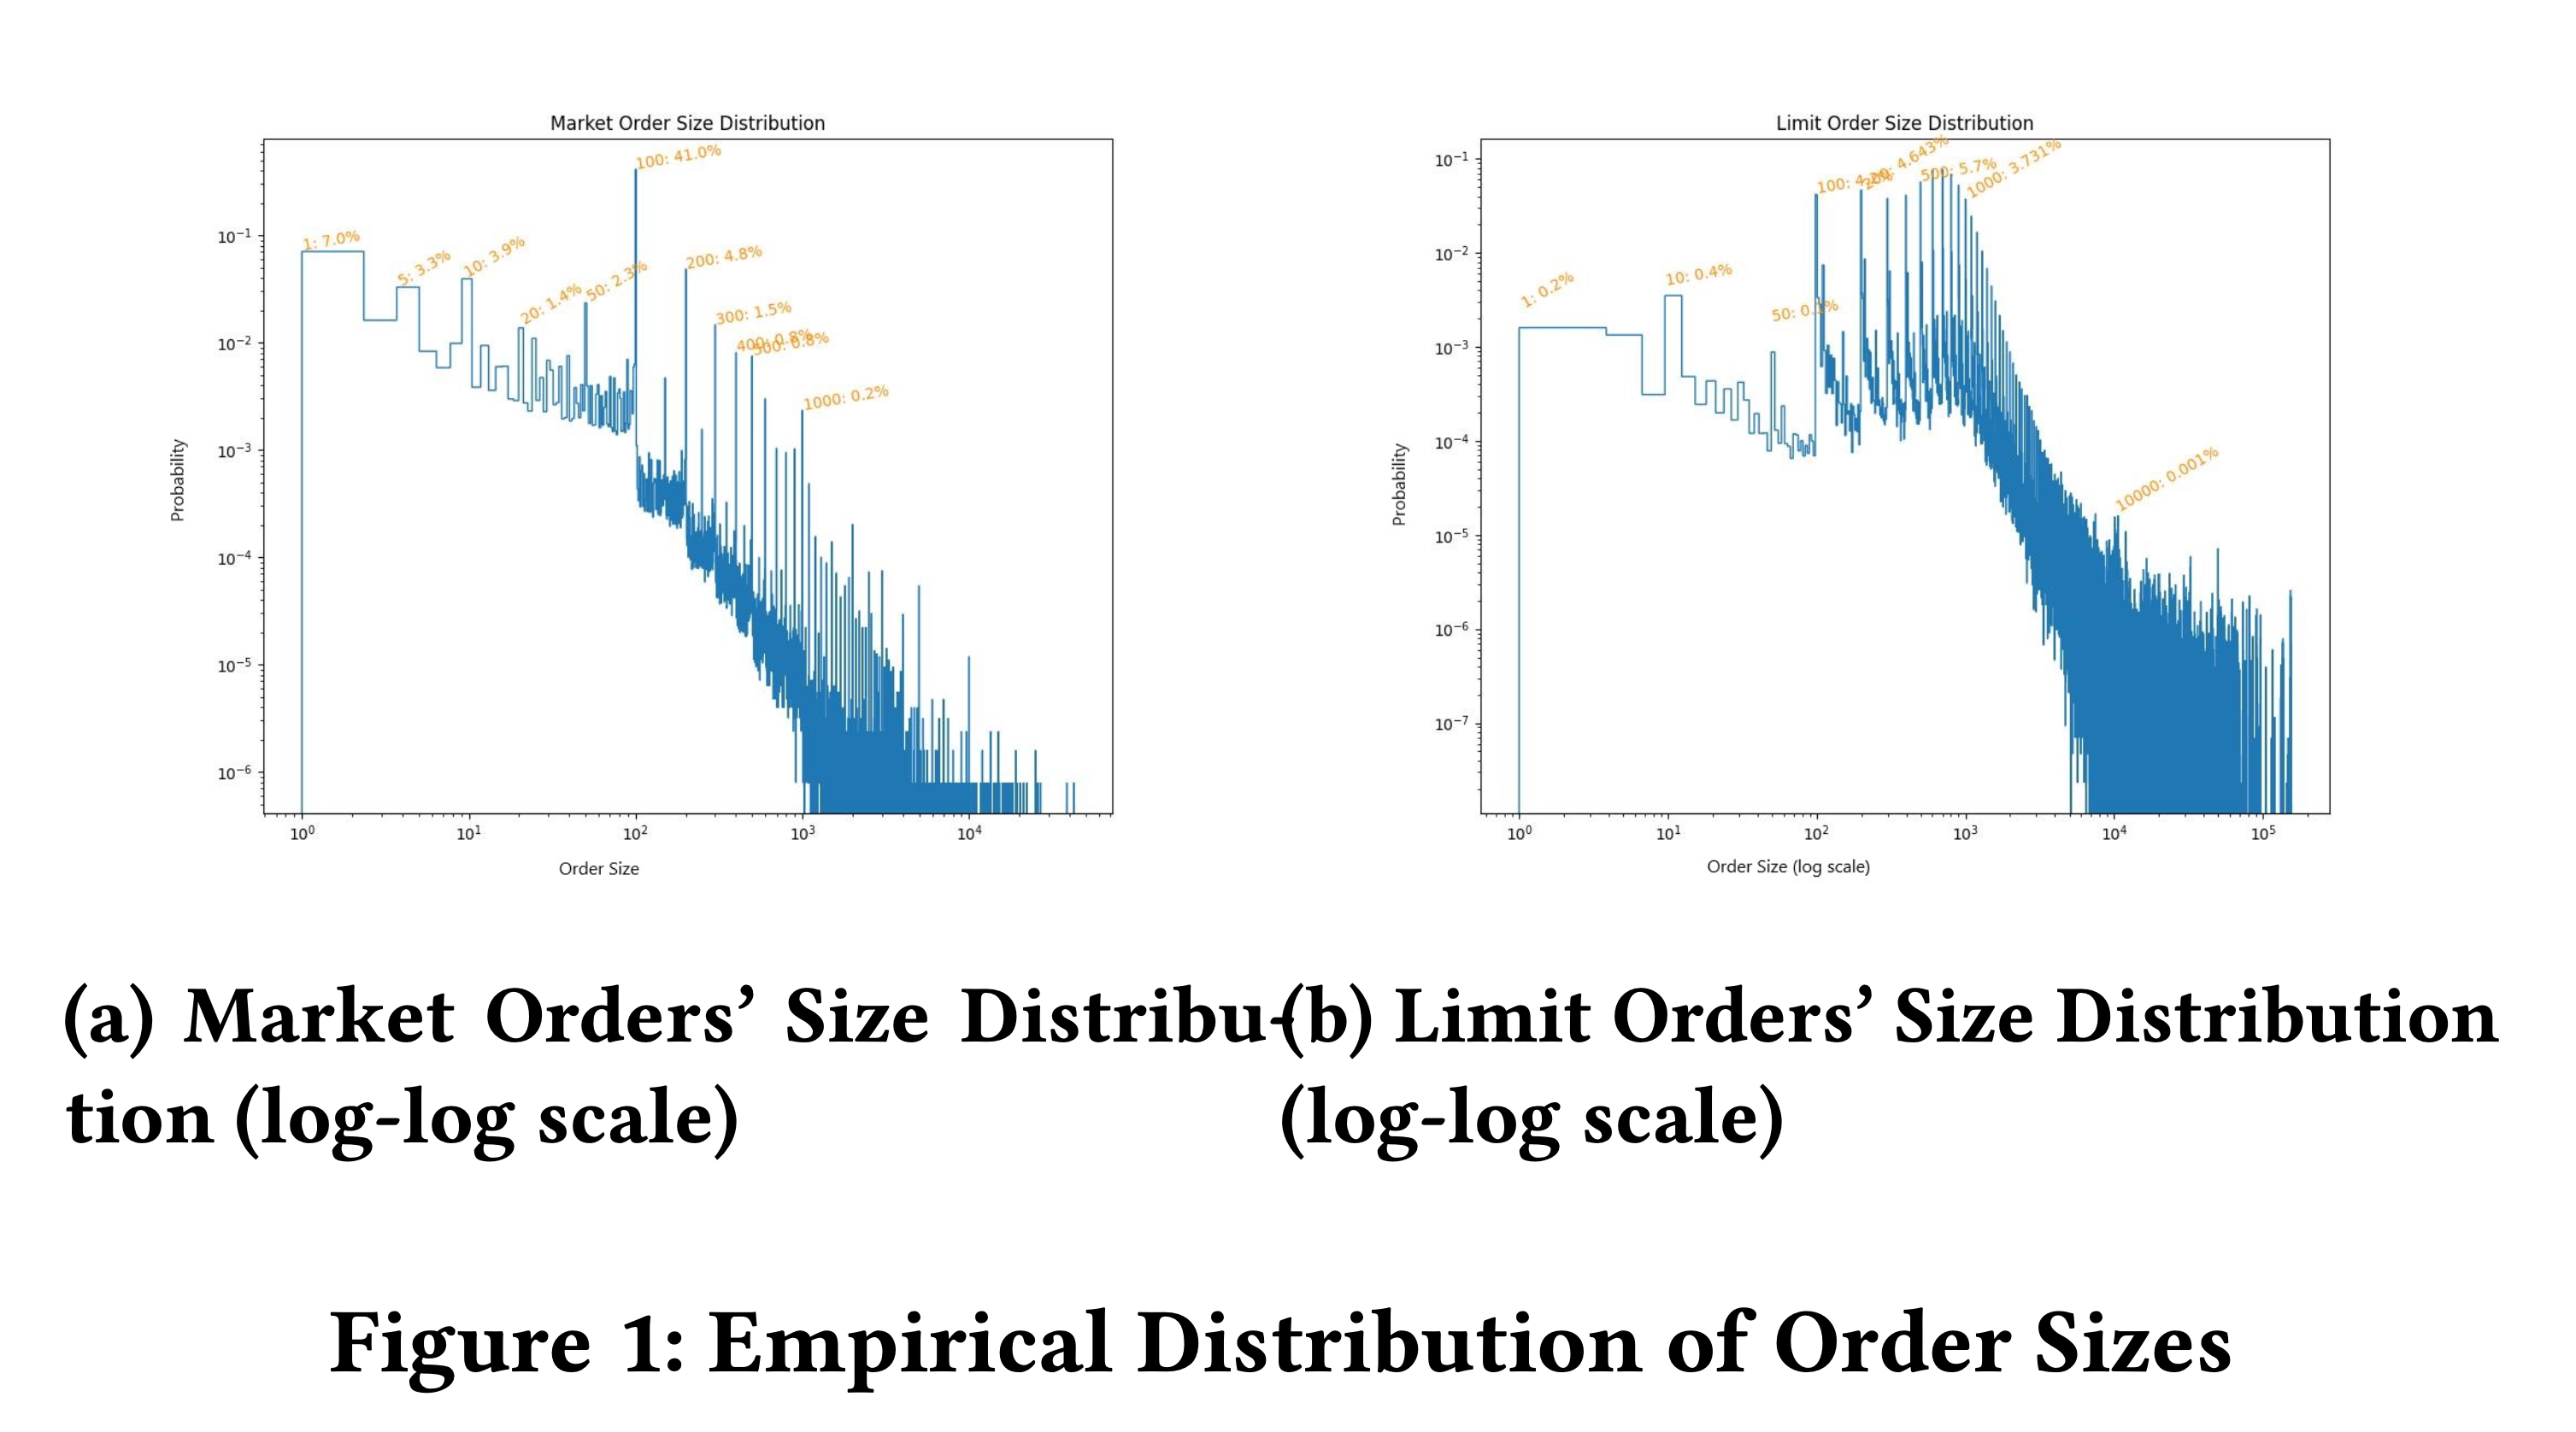
\includegraphics[width=0.82\linewidth]{Screenshot 2026-04-18 at 1.27.42 PM.png}
%     \caption{\textit{(log-log) Empirical Distribution of Order Sizes of 
%     NASDAQ Stocks as given in \cite{jain2023lobhawkes}.}}
%     \label{fig:ordersizespaper}
% \end{figure}
The Compound Hawkes Process, augmented with specific mechanical constraints, effectively resolves these issues by sampling order sizes from a calibrated distribution and dynamically modifying the intensity functions.
\section{Theoretical Framework}

\subsection{The Hawkes Process}

For a $d$-dimensional Hawkes process, the intensity of the process $\lambda^{(i)}(t)$ and its associated counting process $N^{(i)}(t)$ for $i=1,\dots,d$ is defined as:

$$ \lambda^{(i)}(t)=\mu^{(i)}(t)+\sum_{j=1}^{d}\sum_{t_j\in T_j}\phi^{(j\rightarrow i)}(t-t_j) $$

Alternatively, this can be formulated using integrals:

$$ \lambda^{(i)}(t)=\mu^{(i)}(t)+\sum_{j=1}^{d}\int_{0}^{t}\phi^{(j\rightarrow i)}(t-u)dN^{(j)}(u) $$

Where:
\begin{itemize}
    \item $T_j := \{t_j : t_j \le t\}$ is the set of past event times in the $j$-th dimension.
    \item $\mu^{(i)}(t)$ represents the exogenous (baseline) intensity.
    \item $\phi^{(j \rightarrow i)}(t-t_j)$ represents the excitation kernel, a decaying function in time that dictates how an event in dimension $j$ impacts the intensity of dimension $i$.
\end{itemize}

\subsection{The Compound Hawkes Process (CHP)}

A Compound Point Process (CPP) is mathematically defined as:

$$ Z(t)=\sum_{i=1}^{N(t)}Y_i $$

Where $N(t)$ is a counting process with intensity $\lambda(t)$, and $Y_i$ represents independent and identically distributed (i.i.d.) random variables denoting the jump size. A Compound Hawkes Process is a specific case of the CPP where the counting process $N(t)$ is driven by a Hawkes Process. In the context of LOB modelling, $Y_i$ dictates the order size for a specific event type, independently sampled from a calibrated distribution parameterised by $\Theta$.

\section{Simulation Algorithm}

To model the LOB dynamically, the researchers utilized a structured algorithmic approach focusing on the top levels of the book:

\begin{enumerate}
    \item \textbf{Define the State Space:} Formulate the LOB as a 12-dimensional queuing system representing six key queues:
    \begin{center}
        $\{ask_{+1}, ask_0, ask_{-1}, bid_{+1}, bid_0, bid_{-1}\}$
    \end{center}
    The 12 dimensions cover limit orders, market orders, and cancel orders at these respective levels. The subscripts $\pm$ denote the tick distance of the queue from the ask and bid price denoted by '0'.
    \item \textbf{Enforce Mechanical Spread Constraints:} Prevent the spread from becoming negative by formulating the intensities of in-spread limit orders as a function of the current spread. Multiply the intensity by $(s-1)^{\beta}$, ensuring the intensity naturally drops to zero when the spread $s$ is exactly 1 tick.
    \item \textbf{Incorporate Time-of-Day Seasonality:} To capture the ``U''-shape of daily trading volume, model the final intensity as a separable function. Multiply the Hawkes intensity by a piecewise constant function $f^{(i)}(Q_t)$, representing 30-minute bins throughout the trading day.
    \item \textbf{Floor Inhibitory Kernels:} Apply a $\max(0, \dots)$ floor to the total excitation calculation to ensure that inhibitory cross-excitations do not push the point process intensities below zero.
    \item \textbf{Non-Parametric Calibration:} Calibrate the Hawkes kernels non-parametrically using a linear-log spaced time grid, which captures the slow decay of the kernel functions over time.
    \item \textbf{Ensure Process Stability:} Apply constraints during optimization so that the maximum eigenvalue of the kernel norm matrix is limited, ensuring the stationarity and stability of the simulated Hawkes Process.
    \item \textbf{Parametric Fitting:} Fit the resulting non-parametric point estimates to a parametric function. Compare power-law kernels and exponential kernels using the Akaike Information Criterion (AIC), selecting the power-law function $\phi(t) = \alpha(1+\gamma t)^{-\beta}$ for the final simulation.
    \item \textbf{Calibrate Order Sizes:} Calibrate the probability distribution for order sizes using Maximum Likelihood Estimation. Use a geometric distribution combined with Dirac delta functions to insert artificial spikes at standard round numbers (e.g., 10, 50, 100).
    \item \textbf{Simulation:} Utilize the thinning algorithm to generate synthetic order book events based on the finalized, calibrated parameters.
\end{enumerate}

\section{Key Experimental Results}

As per the findings of Jain et al.\cite{jain2023lobhawkes}, the methodology was tested against empirical equity data (such as Apple Inc. on the NASDAQ), yielding several notable results.

\begin{itemize}
    \item \textbf{Replication of Stylized Facts:} The Compound Hawkes Process successfully captures complex microstructural facts, including the shape of the volatility Signature Plot, long auto-correlations of absolute returns, and the long-tailed nature of return distributions.
    \item \textbf{Accurate Spreads and Seasonality:} The explicit spread control mechanism accurately matches empirical spread distributions, while the time-of-day conditioning successfully replicates the ``U''-shape activity seen in real order books.
    \item \textbf{Superiority Over Poisson Models:} When tested against a comparable 12D Compound Poisson model, the Poisson equivalent missed a large mass of inter-arrival time distributions, produced unrealistic spread distributions, and yielded an uncharacteristically flat volatility signature plot.
    \item \textbf{Concave Market Impact:} The simulator organically reproduces a concave relationship between Market Impact (MI) and total order quantity ($Q_T$), aligning with well-known empirical market observations. The simulator also correctly demonstrated that morning trading causes a higher market impact than afternoon trading.
\end{itemize}